\documentclass[tikz,fontsize=8pt]{standalone}
\usepackage{fourier}
\usetikzlibrary{arrows.meta}
\usetikzlibrary{calc}
\tikzset{>=latex}
\definecolor{bookblue}{RGB}{0,173,239}
\definecolor{bookpink}{RGB}{236,0,140}
\definecolor{bookgreen}{RGB}{50,200,0}
\definecolor{bookbluearea}{RGB}{204,239,252}
\tikzstyle{blueline}=[draw=bookblue,line width=0.2mm]
\tikzstyle{pinkline}=[draw=bookpink,line width=0.2mm]
\tikzstyle{greenline}=[draw=bookgreen,line width=0.2mm]
\tikzstyle{blackline}=[draw=black,line width=0.2mm]
\tikzstyle{bluearea}=[fill=bookbluearea]

\usepackage{scrextend}
\changefontsizes[8pt]{8pt}
\usetikzlibrary{decorations.pathreplacing}
\begin{document}
  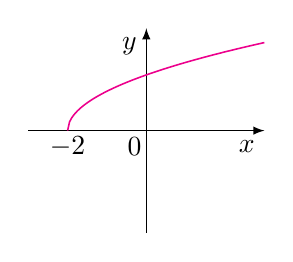
\begin{tikzpicture}
  \node at (-0.15,-0.2) {0};
  \draw[->] (-1.5,0) -- (1.5,0) node[below left] {$x$};
  \draw[->] (0,-1.3) -- (0,1.3) node[below left] {$y$};
  
  \draw[pinkline,domain=0:5,samples=100] plot ({(\x-2)/2},{sqrt(\x)/2});
  %\draw[blueline,domain=0:5,samples=100] plot ({(\x-2)/2},{-sqrt(\x)/2});
  %\fill[bookblue] (-1,0) circle (0.8mm);
  \node at (-1,-0.2) {$-2$};
  \end{tikzpicture}
\end{document}